%\documentclass[13pt]{amsart}
 \documentclass[%
    corpo=12pt,
    twoside,
%    stile=classica,
    oldstyle,
    autoretitolo,
    greek,
    evenboxes,
%    tipotesi,
]{toptesi}
\usepackage{pgfplots}       % it also load tikz package
\pgfplotsset{compat=1.17}   
\usetikzlibrary{arrows.meta}
\usepackage{tikz}
\usetikzlibrary{positioning}
\usepackage{tcolorbox}
\usetikzlibrary{shapes.geometric, arrows, snakes, backgrounds, automata}
\tikzstyle{startstop} = [rectangle, rounded corners, minimum width=3cm, minimum height=1cm,text centered, draw=black, fill=red!30]
\tikzstyle{io} = [trapezium, trapezium left angle=70, trapezium right angle=110, minimum width=1cm, minimum height=1cm, text centered, draw=black, fill=blue!30]
\tikzstyle{process} = [rectangle, minimum width=1cm, minimum height=1cm, text centered, draw=black, fill=orange!30]
\tikzstyle{decision} = [diamond, minimum width=1cm, minimum height=1cm, text centered, draw=black, fill=green!30]
\tikzstyle{arrow} = [thick,->,>=stealth]
%\tikzstyle{state} = [fill=blue!30]
\usepackage{tcolorbox}
\usepackage{caption}
\usepackage[colorlinks=true,
            citecolor={black}]{hyperref}
\usepackage{lipsum} % added for generating a dummy text, 
                    % not needed in real document
\usepackage{fancyvrb}
\begin{document}
\begin{comment}

\section{Ricerca e classificazione delle attestazioni SOA}
\begin{enumerate}
\item identifico una finestra di testo di mio interesse; 
\item all'interno della finestra ricerco istanze delle singole categorie e classifiche;
\item per ogni categoria c individuata, effettuo la normalizzazione normalised\_category(c),
   per cui di quella categoria verrà preso il nome standard;
   ad esempio normalised\_category(\say{og1})  e  normalised\_category(\say{OG 1}) restituiranno entrambe il valore normalizzato \say{OG-1};
\item effettuo un filtraggio sulle categorie finora ottenute:
   se, ad esempio, la regex ammette una categoria come \say{OS-99}, questa non fa parte della lista di categorie SOA "conosciute"   e viene dunque rigettata;
\item effettuo una normalizzazione delle classifiche economiche;
\item concateno categoria SOA e classifica economica trovata; dunque ho a disposizione l'attestazione per intero;
\item per ogni "finestra" di testo, raccolgo le attestazioni individuate e relativi offset (start\_offset, end\_offset) interni al documento;
\item Scrivo l'ouput in un apposito file csv. Per ogni finestra di testo,
   stampo istanze SOA individuate e relative coppie (start\_offset, end\_offset).
\end{enumerate}
L'output di questo prototipo-regex mostra delle limitazioni e dei casi tipici di errore:
in alcune istanze testuali può capitare che una categoria sia menzionata con un nome leggermente diverso da quello canonico (ad es. \say{OS-18}, laddove le alternative accettabili sono \say{OS-18A} e \say{OS-18B}).
In questi casi il filtering, la normalizzazione e anche le regex possono essere leggermente modificate per riconoscere come accettabili tali valori testuali; però modifiche ripetute alle regex possono portare le stesse a diventare incomprensibili e ad essere error-prone.
\end{comment}
\tikzstyle{state}=[circle,draw=blue!50,fill=blue!20,thick]
\tikzstyle{transition}=[rectangle,draw=black!50,fill=black!20,thick]

			
%\filldraw [fill=black!30,draw=red] (semaphore.south -| enter critical.west) rectangle (waiting.north -| leave critical.east);
%REGEX NER
	\begin{figure}[ht] % placed here or on the top of page
		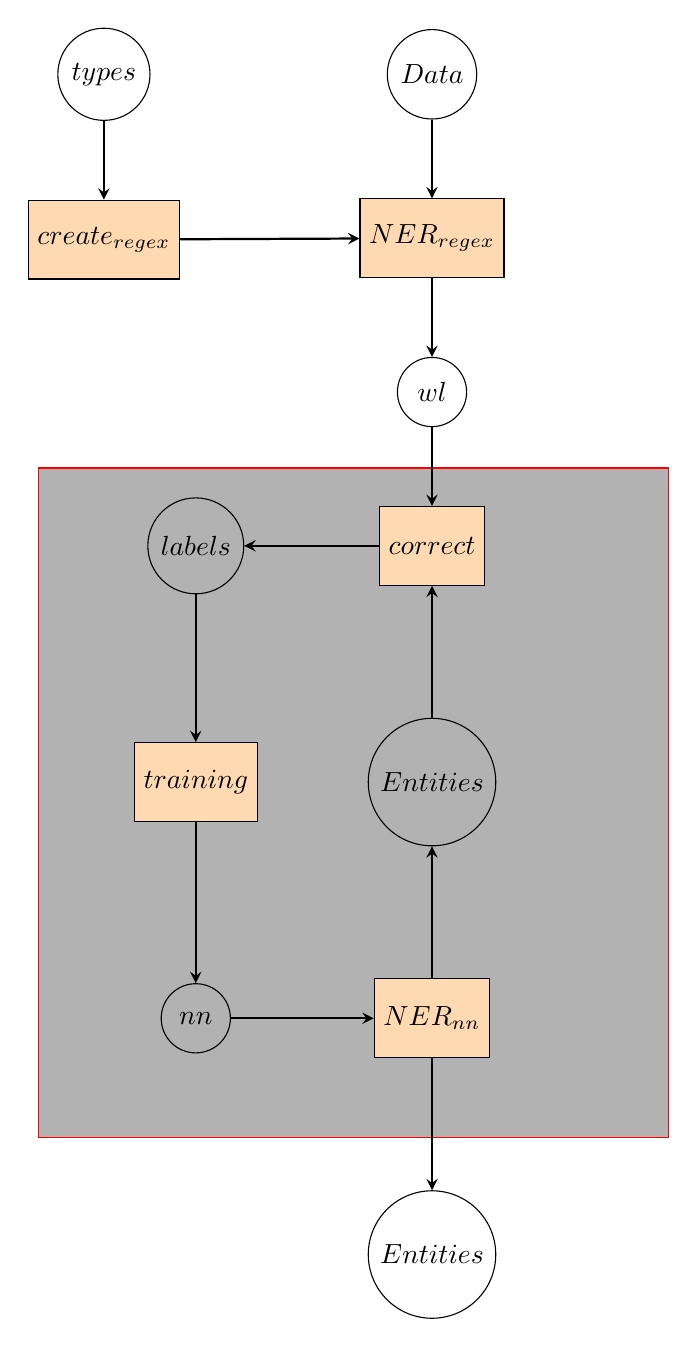
\begin{tikzpicture}[node distance=3cm]
		%\begin{tikzpicture}%[->,shorten >=1pt,auto,node distance=2.8cm,semithick]
			\node (data) [state] {\(Data\)};
			\node (regexner) [process, below=1cm of data] {\(NER\sb{regex}\)};
			\draw [arrow] (data) -- (regexner);
			\node (types) [state, left=3cm of data] {\(types\)};
			\node (humprod) [process, below=1cm of types] {\(create\sb{regex}\)};			
			%\node (regex) [state, left=0.5cm of regexner] {\(R\sb{WL}\)};
			\draw [arrow] (types) -- (humprod);
			\draw [arrow] (humprod) -- (regexner);
			\node (wl) 		[state, below=1cm of regexner] {\(wl\)};
			\draw [arrow] (regexner) -- (wl);
			\node (humcorr) [process, below=1cm of wl] {\(correct\)};
			\draw [arrow] (wl) -- (humcorr);
			\node (l) 		[state, left of=humcorr] {\(labels\)};
			\draw [arrow] (humcorr) -- (l);
			\node (train) 	[process, below of=l] {\(training\)};
			\draw [arrow] (l) -- (train);
			\node (nn) 		[state, below of=train] {\(nn\)};
			\draw [arrow] (train) -- (nn);
			\node (module) [process, right of=nn] {\(NER\sb{nn}\)};
			\draw [arrow] (nn) -- (module);
			\node (entities) [state, below of=module] {\(Entities\)};
			\node (entitiescorr) [state, above of=module] {\(Entities\)};
			\draw [arrow] (module) -- (entities);
			\draw [arrow] (module) -- (entitiescorr);
			\draw [arrow] (entitiescorr) -- (humcorr);
			
\begin{pgfonlayer}{background}
\filldraw [fill=black!30,draw=red] (3,-5) rectangle (-5,-13.5);
%\filldraw [fill=black!30,draw=red] (nn.south -| nn.west) rectangle (humcorr.north -| entitiescorr.east);
\end{pgfonlayer}
		\end{tikzpicture}
%		\caption{Human In The Loop framework} % caption
		%\label{fig:diagram}             % for referencing of figure, key select as you wish
	\end{figure}
%\lipsum[2]  % dummy textù


\end{document}